\documentclass[10pt,twoside,openright,dvipdfmx]{jsbook}

%------------------------------%
% geometry
%------------------------------%

%\usepackage[pass,showframe]{geometry}
\usepackage[pass]{geometry}

%------------------------------%
% afterpage
%------------------------------%

\usepackage{afterpage}
\newcommand\blankpage{%
    \null
    \thispagestyle{empty}
    \addtocounter{page}{-1}
    \newpage
}

%------------------------------%
% makeidx
%------------------------------%

\usepackage{imakeidx}
\makeindex
\indexsetup{othercode={\thispagestyle{plain}}}

%------------------------------%
% fancyhdr
%------------------------------%

\usepackage{fancyhdr}

\pagestyle{fancy}
\fancyhf{}
\fancyhead[RO]{\leftmark}
\fancyhead[LE]{\rightmark}
\fancyfoot[LE,RO]{\thepage}
\setlength{\footskip}{12pt}

% TODO: apply beginning pages of chapter
\fancypagestyle{plain}{%
    \fancyhead{}
    \fancyfoot[LE,RO]{\thepage}
}

%------------------------------%
% color
%------------------------------%

\usepackage{color}
%http://www.biwako.shiga-u.ac.jp/sensei/kumazawa/tex/color.html
\definecolor{ikkonzome}{rgb}	{	0.9961	,	0.7569	,	0.7373	}
\definecolor{ishitake}{rgb}	{	0.9961	,	0.6941	,	0.7059	}
\definecolor{momo}{rgb}	        {	0.9961	,	0.6824	,	0.8039	}
\definecolor{kobai}{rgb}	{	0.9412	,	0.4235	,	0.5569	}
\definecolor{nakabeni}{rgb}	{	0.9451	,	0.2706	,	0.4941	}
\definecolor{sakura}{rgb}	{	0.9333	,	0.8353	,	0.8353	}
\definecolor{arazome}{rgb}	{	0.9725	,	0.7216	,	0.7843	}
\definecolor{usubeni}{rgb}	{	0.8471	,	0.4471	,	0.5451	}
\definecolor{hisame}{rgb}	{	0.7451	,	0.4039	,	0.4039	}
\definecolor{toki}{rgb}	        {	0.9569	,	0.6431	,	0.6353	}
\definecolor{sakuranezumi}{rgb}	{	0.6941	,	0.6039	,	0.6078	}
\definecolor{sango}	{rgb}	{	0.8471	,	0.4157	,	0.3725	}
\definecolor{akane}	{rgb}	{	0.7529	,	0.0118	,	0.3451	}
\definecolor{choshun}{rgb}	{	0.7490	,	0.5255	,	0.5255	}
\definecolor{karakurenai}{rgb}	{	0.7373	,	0.0118	,	0.2667	}
\definecolor{enji}{rgb}	        {	0.6275	,	0.0863	,	0.3176	}
\definecolor{keshiaka}{rgb}	{	0.6275	,	0.4275	,	0.4275	}
\definecolor{kokiake}{rgb}	{	0.5059	,	0.0706	,	0.2549	}
\definecolor{jinzamomi}{rgb}	{	0.9098	,	0.4549	,	0.4157	}
\definecolor{mizugaki}{rgb}	{	0.7294	,	0.5529	,	0.4784	}
\definecolor{umenezumi}{rgb}	{	0.5882	,	0.3922	,	0.3882	}
\definecolor{suoko}{rgb}        {	0.5843	,	0.2667	,	0.2431	}
\definecolor{akabeni}{rgb}	{	0.8039	,	0.0784	,	0.3725	}
\definecolor{shinshu}{rgb}	{	0.6431	,	0.0353	,	0.0000	}
\definecolor{azuki}{rgb}	{	0.5255	,	0.0235	,	0.0000	}
\definecolor{ginshu}{rgb}	{	0.7490	,	0.2824	,	0.0588	}
\definecolor{ebicha}{rgb}	{	0.4549	,	0.2706	,	0.2627	}
\definecolor{kuriume}{rgb}	{	0.5843	,	0.3804	,	0.4314	}
\definecolor{akebono}{rgb}	{	0.8902	,	0.5961	,	0.4941	}
\definecolor{hanezu}{rgb}	{	0.7882	,	0.5961	,	0.5373	}
\definecolor{sangoshu}{rgb}	{	0.8196	,	0.5059	,	0.4471	}
\definecolor{shozyohi}{rgb}	{	0.7686	,	0.0000	,	0.0000	}
\definecolor{shikancha}{rgb}	{	0.5569	,	0.3294	,	0.1882	}
\definecolor{kakishibu}{rgb}	{	0.6745	,	0.4078	,	0.3333	}
\definecolor{benikaba}{rgb}	{	0.7137	,	0.3373	,	0.2941	}
\definecolor{benitobi}{rgb}	{	0.6196	,	0.3176	,	0.2706	}
\definecolor{benihihada}{rgb}	{	0.5020	,	0.3137	,	0.2353	}
\definecolor{kurotobi}{rgb}	{	0.3176	,	0.2000	,	0.1490	}
\definecolor{benihi}{rgb}	{	0.8235	,	0.4745	,	0.1922	}
\definecolor{terigaki}{rgb}	{	0.8118	,	0.4627	,	0.1804	}
\definecolor{ake}{rgb}	        {	0.7804	,	0.3098	,	0.1725	}
\definecolor{edocha}{rgb}	{	0.6863	,	0.4353	,	0.2941	}
\definecolor{bengara}{rgb}	{	0.6392	,	0.1569	,	0.0196	}
\definecolor{hihada}{rgb}	{	0.5412	,	0.3412	,	0.2353	}
\definecolor{shishi}{rgb}	{	0.8549	,	0.6863	,	0.5961	}
\definecolor{araishu}{rgb}	{	0.9294	,	0.4902	,	0.4549	}
\definecolor{akago}{rgb}	{	0.8118	,	0.5765	,	0.4275	}
\definecolor{tokigaracha}{rgb}	{	0.7922	,	0.5255	,	0.3686	}
\definecolor{otan}{rgb}	        {	0.8157	,	0.4157	,	0.2235	}
\definecolor{komugi}{rgb}	{	0.8157	,	0.6549	,	0.5098	}
\definecolor{rakuda}{rgb}	{	0.6784	,	0.5255	,	0.4118	}
\definecolor{tsurubami}{rgb}	{	0.6275	,	0.4392	,	0.3961	}
\definecolor{ama}{rgb}	        {	0.7765	,	0.6902	,	0.5843	}
\definecolor{nikkei}{rgb}	{	0.7216	,	0.4667	,	0.3725	}
\definecolor{renga}{rgb}	{	0.6902	,	0.3765	,	0.3098	}
\definecolor{sohi}{rgb}   	{	0.8078	,	0.5098	,	0.2078	}
\definecolor{enshucha}{rgb}	{	0.6706	,	0.4275	,	0.1608	}
\definecolor{karacha}{rgb}	{	0.5765	,	0.4235	,	0.1490	}
\definecolor{kabacha}{rgb}	{	0.6353	,	0.3725	,	0.1569	}
\definecolor{sodenkaracha}{rgb}	{	0.5216	,	0.3490	,	0.1373	}
\definecolor{suzumecha}{rgb}	{	0.4745	,	0.3176	,	0.1255	}
\definecolor{kurikawacha}{rgb}	{	0.4078	,	0.2745	,	0.1098	}
\definecolor{momoshiocha}{rgb}	{	0.3490	,	0.2353	,	0.0902	}
\definecolor{tobi}{rgb}	        {	0.4353	,	0.3098	,	0.1412	}
\definecolor{kurumizome}{rgb}	{	0.6667	,	0.5333	,	0.3333	}
\definecolor{kaba}{rgb}	        {	0.8196	,	0.4588	,	0.1294	}
\definecolor{korosen}{rgb}	{	0.5059	,	0.3843	,	0.1608	}
\definecolor{kogecha}{rgb}	{	0.3333	,	0.2549	,	0.1098	}
\definecolor{kokikuchinashi}{rgb}	{	0.8078	,	0.5922	,	0.3490	}
\definecolor{araigaki}{rgb}	{	0.8157	,	0.5529	,	0.3176	}
\definecolor{taisha}{rgb}	{	0.6353	,	0.4196	,	0.2078	}
\definecolor{akashirotsurubami}{rgb}	{	0.8078	,	0.6118	,	0.4157	}
\definecolor{tonocha}{rgb}	{	0.5922	,	0.4039	,	0.2000	}
\definecolor{sencha}{rgb}	{	0.5255	,	0.3529	,	0.1490	}
\definecolor{sharegaki}{rgb}	{	0.8549	,	0.7098	,	0.4863	}
\definecolor{ko}{rgb}	        {	0.9529	,	0.8275	,	0.6627	}
\definecolor{usugaki}{rgb}	{	0.8627	,	0.7294	,	0.5294	}
\definecolor{koji}{rgb}	        {	0.8275	,	0.6039	,	0.2706	}
\definecolor{umezome}{rgb}	{	0.8667	,	0.7373	,	0.4235	}
\definecolor{beniukon}{rgb}	{	0.8549	,	0.5843	,	0.2549	}
\definecolor{chojicha}{rgb}	{	0.5569	,	0.4000	,	0.1098	}
\definecolor{kenpozome}{rgb}	{	0.3059	,	0.2667	,	0.0627	}
\definecolor{biwacha}{rgb}	{	0.7333	,	0.5294	,	0.1922	}
\definecolor{kohaku}{rgb}	{	0.8039	,	0.5961	,	0.2471	}
\definecolor{usuko}{rgb}	{	0.8745	,	0.7373	,	0.4824	}
\definecolor{kuchiba}{rgb}	{	0.8157	,	0.6157	,	0.3216	}
\definecolor{kincha}{rgb}	{	0.7725	,	0.4902	,	0.2000	}
\definecolor{chozizome}{rgb}	{	0.5686	,	0.3961	,	0.1608	}
\definecolor{kitsune}{rgb}	{	0.6392	,	0.4431	,	0.1804	}
\definecolor{hushizome}{rgb}	{	0.5804	,	0.4353	,	0.1608	}
\definecolor{kyara}{rgb}	{	0.4510	,	0.3373	,	0.1255	}
\definecolor{susutake}{rgb}	{	0.4588	,	0.3529	,	0.1176	}
\definecolor{shirocha}{rgb}	{	0.7529	,	0.6588	,	0.4118	}
\definecolor{odo}{rgb}	        {	0.7137	,	0.6039	,	0.3137	}
\definecolor{ginsusutake}{rgb}	{	0.5608	,	0.4745	,	0.2392	}
\definecolor{kigaracha}{rgb}	{	0.7490	,	0.6196	,	0.2745	}
\definecolor{kobicha}	{rgb}	{	0.5020	,	0.4118	,	0.1765	}
\definecolor{usuki}	{rgb}	{	0.8549	,	0.7804	,	0.4275	}
\definecolor{yamabuki}	{rgb}	{	0.9098	,	0.8000	,	0.2039	}
\definecolor{tamago}	{rgb}	{	0.8275	,	0.7412	,	0.3373	}
\definecolor{hajizome}	{rgb}	{	0.7412	,	0.6039	,	0.2431	}
\definecolor{yamabukicha}{rgb}	{	0.7059	,	0.5765	,	0.2275	}
\definecolor{kuwazome}	{rgb}	{	0.6471	,	0.5255	,	0.2118	}
\definecolor{namakabe}	{rgb}	{	0.5569	,	0.4549	,	0.1843	}
\definecolor{kuchinashi}{rgb}	{	0.8078	,	0.7333	,	0.3843	}
\definecolor{tomorokoshi}{rgb}	{	0.7804	,	0.7020	,	0.2941	}
\definecolor{shirotsurubami}{rgb}	{	0.8745	,	0.8235	,	0.5922	}
\definecolor{kitsurubami}{rgb}	{	0.6863	,	0.6039	,	0.2118	}
\definecolor{toou}	{rgb}	{	0.8353	,	0.7725	,	0.4235	}
\definecolor{hanaba}	{rgb}	{	0.8549	,	0.8000	,	0.4941	}
\definecolor{torinoko}	{rgb}	{	0.8431	,	0.8118	,	0.6902	}
\definecolor{ukon}	{rgb}	{	0.8039	,	0.7216	,	0.3059	}
\definecolor{kikuchiba}	{rgb}	{	0.7765	,	0.6667	,	0.2902	}
\definecolor{rikyushiracha}{rgb}{	0.6627	,	0.6471	,	0.4784	}
\definecolor{rikyucha}	{rgb}	{	0.5176	,	0.5176	,	0.2588	}
\definecolor{aku}	{rgb}	{	0.5294	,	0.5059	,	0.4039	}
\definecolor{higosusutake}{rgb}	{	0.4863	,	0.4510	,	0.3059	}
\definecolor{rokocha}	{rgb}	{	0.4157	,	0.4353	,	0.3686	}
\definecolor{mirucha}	{rgb}	{	0.4471	,	0.4471	,	0.3725	}
\definecolor{natane}	{rgb}	{	0.7216	,	0.6863	,	0.3882	}
\definecolor{kimirucha}	{rgb}	{	0.5373	,	0.5059	,	0.2549	}
\definecolor{uguisucha}	{rgb}	{	0.4118	,	0.3882	,	0.1961	}
\definecolor{nanohana}	{rgb}	{	0.9882	,	0.9882	,	0.3804	}
\definecolor{kariyasu}	{rgb}	{	0.8039	,	0.7686	,	0.3882	}
\definecolor{kihada}	{rgb}	{	0.9608	,	0.9137	,	0.2863	}
\definecolor{zoge}	{rgb}	{	0.8863	,	0.8235	,	0.7216	}
\definecolor{wara}	{rgb}	{	0.7882	,	0.7490	,	0.4706	}
\definecolor{macha}	{rgb}	{	0.6235	,	0.6392	,	0.4863	}
\definecolor{yamabato}	{rgb}	{	0.5137	,	0.5176	,	0.4000	}
\definecolor{mushikuri}	{rgb}	{	0.8196	,	0.8000	,	0.6118	}
\definecolor{aokuchiba}	{rgb}	{	0.6275	,	0.6392	,	0.3451	}
\definecolor{hiwacha}	{rgb}	{	0.6784	,	0.6863	,	0.4196	}
\definecolor{ominaeshi}	{rgb}	{	0.8745	,	0.8863	,	0.4039	}
\definecolor{wasabi}	{rgb}	{	0.5922	,	0.6824	,	0.5765	}
\definecolor{uguisu}	{rgb}	{	0.3333	,	0.4118	,	0.0627	}
\definecolor{hiwa}	{rgb}	{	0.7098	,	0.7216	,	0.2392	}
\definecolor{aoshirotsurubami}{rgb}	{	0.5961	,	0.6471	,	0.4471	}
\definecolor{yanagicha}	{rgb}	{	0.5373	,	0.5725	,	0.3529	}
\definecolor{rikancha}	{rgb}	{	0.3333	,	0.4196	,	0.2863	}
\definecolor{aikobicha}	{rgb}	{	0.2706	,	0.3412	,	0.2353	}
\definecolor{koke}	{rgb}	{	0.4941	,	0.5686	,	0.3922	}
\definecolor{miru}	{rgb}	{	0.1529	,	0.3216	,	0.1843	}
\definecolor{sensai}	{rgb}	{	0.1373	,	0.2863	,	0.1608	}
\definecolor{baiko}	{rgb}	{	0.5529	,	0.6157	,	0.3922	}
\definecolor{iwai}	{rgb}	{	0.3059	,	0.4118	,	0.2784	}
\definecolor{hiwamoegi}	{rgb}	{	0.4431	,	0.6824	,	0.2431	}
\definecolor{yanagisusutake}{rgb}	{	0.2039	,	0.3333	,	0.1255	}
\definecolor{urayanagi}	{rgb}	{	0.5843	,	0.6824	,	0.2431	}
\definecolor{usumoegi}	{rgb}	{	0.4824	,	0.6706	,	0.2275	}
\definecolor{yanagizome}{rgb}	{	0.4353	,	0.6000	,	0.2078	}
\definecolor{moegi}	{rgb}	{	0.3020	,	0.5961	,	0.1882	}
\definecolor{aoni}	{rgb}	{	0.1216	,	0.4196	,	0.2431	}
\definecolor{matsuba}	{rgb}	{	0.1098	,	0.3686	,	0.2118	}
\definecolor{usuao}	{rgb}	{	0.5529	,	0.7059	,	0.6118	}
\definecolor{wakatake}	{rgb}	{	0.3843	,	0.6824	,	0.5059	}
\definecolor{yanaginezumi}{rgb}	{	0.5020	,	0.6078	,	0.5490	}
\definecolor{oitake}	{rgb}	{	0.4157	,	0.5412	,	0.4392	}
\definecolor{sensaimidori}{rgb}	{	0.2549	,	0.3882	,	0.2627	}
\definecolor{midori}	{rgb}	{	0.0000	,	0.4824	,	0.0000	}
\definecolor{byakuroku}	{rgb}	{	0.6078	,	0.7333	,	0.6196	}
\definecolor{sabiseiji}	{rgb}	{	0.5333	,	0.6588	,	0.5804	}
\definecolor{rokusho}	{rgb}	{	0.3373	,	0.6039	,	0.4039	}
\definecolor{tokusa}	{rgb}	{	0.2549	,	0.4706	,	0.3922	}
\definecolor{onandocha}	{rgb}	{	0.2039	,	0.3725	,	0.3098	}
\definecolor{aotake}	{rgb}	{	0.1412	,	0.5176	,	0.4353	}
\definecolor{rikyunezumi}{rgb}	{	0.4157	,	0.5686	,	0.5490	}
\definecolor{birodo}	{rgb}	{	0.1059	,	0.4275	,	0.3608	}
\definecolor{mishiao}	{rgb}	{	0.1098	,	0.4588	,	0.3882	}
\definecolor{aimirucha}	{rgb}	{	0.2510	,	0.4000	,	0.3608	}
\definecolor{tonotya}	{rgb}	{	0.3059	,	0.4941	,	0.4392	}
\definecolor{mizuasagi}	{rgb}	{	0.1569	,	0.6745	,	0.6745	}
\definecolor{seji}	{rgb}	{	0.4745	,	0.6588	,	0.5922	}
\definecolor{seheki}	{rgb}	{	0.0588	,	0.5569	,	0.4824	}
\definecolor{sabitetsu}	{rgb}	{	0.0392	,	0.3294	,	0.2784	}
\definecolor{tetsu}	{rgb}	{	0.0627	,	0.3961	,	0.3961	}
\definecolor{omeshicha}	{rgb}	{	0.0667	,	0.4667	,	0.4667	}
\definecolor{korainando}{rgb}	{	0.0588	,	0.3922	,	0.0392	}
\definecolor{minatonezumi}{rgb}	{	0.4549	,	0.6000	,	0.6118	}
\definecolor{aonibi}	{rgb}	{	0.1804	,	0.3725	,	0.3882	}
\definecolor{tetsuonando}{rgb}	{	0.1961	,	0.4118	,	0.4275	}
\definecolor{mizu}	{rgb}	{	0.5451	,	0.7412	,	0.7608	}
\definecolor{sabiasagi}	{rgb}	{	0.4510	,	0.6000	,	0.6000	}
\definecolor{kamenozoki}{rgb}	{	0.7098	,	0.9020	,	0.8902	}
\definecolor{asagi}	{rgb}	{	0.3020	,	0.6784	,	0.7098	}
\definecolor{shinbashi}	{rgb}	{	0.0000	,	0.6000	,	0.6353	}
\definecolor{sabionando}{rgb}	{	0.2392	,	0.3961	,	0.3843	}
\definecolor{ainezumi}	{rgb}	{	0.2235	,	0.4000	,	0.3843	}
\definecolor{ai}	{rgb}	{	0.2039	,	0.3765	,	0.4314	}
\definecolor{onando}	{rgb}	{	0.1843	,	0.3686	,	0.4000	}
\definecolor{hanaasagi}	{rgb}	{	0.2000	,	0.6196	,	0.7098	}
\definecolor{chigusa}	{rgb}	{	0.1922	,	0.5725	,	0.6745	}
\definecolor{masuhana}	{rgb}	{	0.1569	,	0.4667	,	0.5569	}
\definecolor{hanada}	{rgb}	{	0.0039	,	0.4275	,	0.5373	}
\definecolor{noshimehana}{rgb}	{	0.1412	,	0.4235	,	0.5098	}
\definecolor{omeshionando}{rgb}	{	0.1176	,	0.3529	,	0.4235	}
\definecolor{sora}	{rgb}	{	0.1451	,	0.7216	,	0.8039	}
\definecolor{konpeki}	{rgb}	{	0.0902	,	0.5098	,	0.7333	}
\definecolor{kurotsurubami}{rgb}{	0.0627	,	0.3137	,	0.3451	}
\definecolor{gunjo}	{rgb}	{	0.5098	,	0.7882	,	0.9098	}
\definecolor{kon}	{rgb}	{	0.0000	,	0.2000	,	0.4000	}
\definecolor{kachi}	{rgb}	{	0.0000	,	0.1765	,	0.3490	}
\definecolor{ruri}	{rgb}	{	0.0078	,	0.3922	,	0.6510	}
\definecolor{konjo}	{rgb}	{	0.0039	,	0.3137	,	0.5216	}
\definecolor{rurikon}	{rgb}	{	0.0000	,	0.3020	,	0.5020	}
\definecolor{benimidori}{rgb}	{	0.3373	,	0.4588	,	0.6784	}
\definecolor{konkikyo}	{rgb}	{	0.0039	,	0.0667	,	0.4275	}
\definecolor{hujinezumi}{rgb}	{	0.3216	,	0.3686	,	0.6118	}
\definecolor{benikakehana}{rgb}	{	0.2275	,	0.2471	,	0.5882	}
\definecolor{hujiiro}	{rgb}	{	0.4706	,	0.4863	,	0.7059	}
\definecolor{hutaai}	{rgb}	{	0.3137	,	0.3333	,	0.5608	}
\definecolor{hujimurasaki}{rgb}	{	0.4157	,	0.3333	,	0.5686	}
\definecolor{kikyo}	{rgb}	{	0.3529	,	0.3216	,	0.5725	}
\definecolor{shion}	{rgb}	{	0.5137	,	0.4196	,	0.6784	}
\definecolor{messhi}	{rgb}	{	0.2196	,	0.1765	,	0.3098	}
\definecolor{shikon}	{rgb}	{	0.2510	,	0.1961	,	0.3529	}
\definecolor{kokimurasaki}{rgb}	{	0.3098	,	0.2000	,	0.3765	}
\definecolor{usu}	{rgb}	{	0.7294	,	0.6353	,	0.7843	}
\definecolor{hashita}	{rgb}	{	0.6000	,	0.4549	,	0.6706	}
\definecolor{rindo}	{rgb}	{	0.5922	,	0.5137	,	0.7529	}
\definecolor{sumire}	{rgb}	{	0.3882	,	0.2157	,	0.5922	}
\definecolor{nasukon}	{rgb}	{	0.3216	,	0.2235	,	0.4353	}
\definecolor{murasaki}	{rgb}	{	0.3137	,	0.1765	,	0.4824	}
\definecolor{kurobeni}	{rgb}	{	0.2353	,	0.1294	,	0.3059	}
\definecolor{ayame}	{rgb}	{	0.4275	,	0.1569	,	0.5098	}
\definecolor{benihuji}	{rgb}	{	0.6824	,	0.5333	,	0.6667	}
\definecolor{edomurasaki}{rgb}	{	0.3961	,	0.1529	,	0.4392	}
\definecolor{kodaimurasaki}{rgb}{	0.4353	,	0.2863	,	0.4627	}
\definecolor{shikon}{rgb}       {	0.4118	,	0.2549	,	0.3765	}
\definecolor{hatobanezumi}{rgb}	{	0.4235	,	0.3804	,	0.4392	}
\definecolor{budonezumi}{rgb}	{	0.3412	,	0.2196	,	0.3529	}
\definecolor{ebizome}	{rgb}	{	0.4000	,	0.2235	,	0.3882	}
\definecolor{hujisusutake}{rgb}	{	0.2549	,	0.0824	,	0.2471	}
\definecolor{usuebi}	{rgb}	{	0.6549	,	0.4392	,	0.6039	}
\definecolor{botan}	{rgb}	{	0.6706	,	0.0392	,	0.4353	}
\definecolor{umemurasaki}{rgb}	{	0.6667	,	0.3922	,	0.5176	}
\definecolor{nisemurasaki}{rgb}	{	0.3686	,	0.0000	,	0.3216	}
\definecolor{murasakitobi}{rgb}	{	0.3922	,	0.3255	,	0.3529	}
\definecolor{ususuo}{rgb}	{	0.7569	,	0.4000	,	0.5412	}
\definecolor{suo}{rgb}	        {	0.6941	,	0.0627	,	0.4157	}
\definecolor{kuwanomi}{rgb}	{	0.4196	,	0.0549	,	0.2745	}
\definecolor{nibi}{rgb}	        {	0.4549	,	0.4235	,	0.3961	}
\definecolor{benikeshi}{rgb}	{	0.4118	,	0.3804	,	0.3843	}
\definecolor{shironeri}{rgb}	{	0.9843	,	0.9843	,	0.9843	}
\definecolor{shironezumi}{rgb}	{	0.6471	,	0.6588	,	0.6627	}
\definecolor{ginnezumi}{rgb}	{	0.5255	,	0.5490	,	0.5922	}
\definecolor{sunezumi}{rgb}	{	0.4275	,	0.4392	,	0.4392	}
\definecolor{dobunezumi}{rgb}	{	0.2863	,	0.2941	,	0.2941	}
\definecolor{aisumicha}{rgb}	{	0.2078	,	0.2196	,	0.2510	}
\definecolor{binrojizome}{rgb}	{	0.2118	,	0.0824	,	0.0706	}
\definecolor{sumizome}{rgb}	{	0.2706	,	0.2706	,	0.2706	}


%------------------------------%
% graphicx
%------------------------------%

\usepackage{graphicx}

%------------------------------%
% listings
%------------------------------%

\usepackage{listings,jlisting}
\lstdefinelanguage{swift}{
    sensitive=true,
    keywords=[1]{associatedtype,class,deinit,enum,extension,fileprivate,func,import,init,inout,internal,let,open,operator,private,protocol,public,static,struct,subscript,typealias,var,break,case,continue,default,defer,do,else,fallthrough,for,guard,if,in,repeat,return,switch,where,while,as,Any,catch,false,is,nil,rethrows,super,self,Self,throw,throws,true,try,\_,associativity,convenience,dynamic,didSet,final,get,infix,indirect,lazy,left,mutating,none,nonmutating,optional,override,postfix,precedence,prefix,Protocol,required,right,set,Type,unowned,weak,willSet},
    keywords=[2]{\#available,\#colorLiteral,\#column,\#else,\#elseif,\#endif,\#file,\#fileLiteral,\#function,\#if,\#imageLiteral,\#line,\#selector,\#sourceLocation},
    numbers=left,
    numberstyle=\scriptsize,
    stepnumber=1,
    numbersep=8pt,
    showstringspaces=false,
    breaklines=true,
    morecomment=[l]{//},
    morecomment=[s]{/*}{*/},
    keywordstyle=[1]\color{konpeki},
    keywordstyle=[2]\color{konjo},
    commentstyle=\color{usumoegi},
    stringstyle=\color{enji},
    morestring=[b]",%"
}

\renewcommand{\lstlistingname}{プログラム}
\lstset{language=swift,
    basicstyle=\ttfamily\scriptsize,
    commentstyle=\textit,
    classoffset=1,
    keywordstyle=\bfseries,
    frame=tRBl,
    framesep=5pt,
    showstringspaces=false,
    numbers=left,
    stepnumber=1,
    numberstyle=\tiny,
    tabsize=2
}


\lstdefinelanguage{objectivec}{
    sensitive=true,
    keywords=[1]{auto,break,case,char,const,continue,default,do,double,else,enum,extern,float,for,goto,if,inline,int,long,register,restrict,return,short,signed,sizeof,static,struct,switch,typedef,union,unsigned,void,volatile,while,\_Bool,\_Complex,\_Imaginary,BOOL,Class,bycopy,byref,id,IMP,in,inout,nil,NO,NULL,oneway,out,Protocol,SEL,self,super,YES,@interface,@end,@implementation,@protocol,@class,@public,@protected,@private,@property,@try,@throw,@catch,@finally,@synthesize,@dynamic,@selector,atomic,nonatomic,retain},
    keywords=[2]{\#define,\#include,\#undef,\#ifdef,\#ifndef,\#if,\#else,\#elif,\#endif,\#error,\#import,\#pragma},
    numbers=left,
    numberstyle=\scriptsize,
    stepnumber=1,
    numbersep=8pt,
    showstringspaces=false,
    breaklines=true,
    morecomment=[l]{//},
    morecomment=[s]{/*}{*/},
    keywordstyle=[1]\color{konpeki},
    keywordstyle=[2]\color{rindo},
    commentstyle=\color{usumoegi},
    stringstyle=\color{enji},
    morestring=[b]",%"
}

\renewcommand{\lstlistingname}{プログラム}
\lstset{language=swift,
    basicstyle=\ttfamily\scriptsize,
    commentstyle=\textit,
    classoffset=1,
    keywordstyle=\bfseries,
    frame=tRBl,
    framesep=5pt,
    showstringspaces=false,
    numbers=left,
    stepnumber=1,
    numberstyle=\tiny,
    tabsize=2
}


\lstdefinelanguage{javascript}{
    sensitive=true,
    keywords=[1]{class,export,boolean,throw,implements,import,this,typeof,new,true,false,catch,function,return,null,catch,switch,var,if,in,while,do,else,case,break},
    keywords=[2]{},
    numbers=left,
    numberstyle=\scriptsize,
    stepnumber=1,
    numbersep=8pt,
    showstringspaces=false,
    breaklines=true,
    morecomment=[l]{//},
    morecomment=[s]{/*}{*/},
    keywordstyle=[1]\color{konpeki},
    keywordstyle=[2]\color{rindo},
    commentstyle=\color{usumoegi},
    stringstyle=\color{enji},
    identifierstyle=\color{black},
    morestring=[b]',
    morestring=[b]"
}

\renewcommand{\lstlistingname}{プログラム}
\lstset{language=javascript,
    basicstyle=\ttfamily\scriptsize,
    commentstyle=\textit,
    classoffset=1,
    keywordstyle=\bfseries,
    frame=tRBl,
    framesep=5pt,
    showstringspaces=false,
    numbers=left,
    stepnumber=1,
    numberstyle=\tiny,
    tabsize=2
}



%------------------------------%
% box
%------------------------------%

\usepackage{ascmac,fancybox}

%------------------------------%
% appendix
%------------------------------%

\usepackage[toc,page]{appendix}

\makeatletter
\AtBeginEnvironment{appendices}{%
  \clearpage%
  \fancypagestyle{plain}{%
    \fancyhf{}%
    \renewcommand{\headrulewidth}{0pt}
  }
  \thispagestyle{plain}
}

%------------------------------%
% biblatex
%------------------------------%

\usepackage[style=numeric,backend=biber,defernumbers=true]{biblatex}
\addbibresource{bibliographies/apple.bib}
\addbibresource{bibliographies/articles.bib}
\addbibresource{bibliographies/others.bib}

%------------------------------%
% accented letters
%------------------------------%

\usepackage[utf8]{inputenc}

%------------------------------%
% development
%------------------------------%

\usepackage{lipsum}
\usepackage{layout}

%------------------------------%
% title
%------------------------------%

\usepackage{authblk}

\title{%
    先生,まだテスト習ってません(仮) \\
    \large iOSDC2017草稿}
\author[$\dagger$]{しもとりしぐれ}
\affil[$\dagger$]{@S\_Shimotori}
\date{\today}

%------------------------------%
% hyperref
%------------------------------%

\usepackage[colorlinks]{hyperref}

\hypersetup{
    urlcolor=hujinezumi,
    citecolor=sora,
    linkcolor=black
}

\usepackage[normalem]{ulem}

\makeatletter
\begingroup
    \catcode`\$=6
    \catcode`\#=12
    \gdef\href@split$1#$2#$3\\$4{
        \hyper@@link{$1}{$2}{\uline{$4}}
        \endgroup
    }%
\endgroup

%------------------------------%
% document
%------------------------------%

\begin{document}

\pagenumbering{Alph}
\newgeometry{hmarginratio=1:1}
\maketitle
\restoregeometry

\afterpage{\blankpage}

\pagenumbering{roman}

\tableofcontents
\thispagestyle{plain}

\chapter*{はしがき}
\thispagestyle{plain}
\addcontentsline{toc}{chapter}{はしがき}
勉強会や懇親会では,しばしば「テストを書いていますか?」という会話が行われます.その回答に耳を傾けると,

\begin{screen}%
\noindent 「書いてないんですよね」 \\
「モデルのテストなら書いてます」 \\
「JUnitなら授業で習ったけど」 \\
「ユニットテストだけ書いてれば十分じゃないかな」 \\
「書いたことないです」
\end{screen}

\noindent というネガティブなものが目立ちます.上2つは社会人の方の,下3つは学生の方の実際の回答です.特に学生や新社会人をはじめとする初心者の方に憂慮を覚えるところでしょう.なぜならテストを学ぶ機会とモチベーションは限られているからです.筆者の大学では,テストを含む開発手法の授業は必修ではありません.必修の学校があったとしても,プログラミングパラダイムやアルゴリズム,データ構造を学んで余った時間で行われることでしょう.また,インターネット上には新卒に書籍を勧めるブログ記事が多々ありますが,そのリストの中にテストに関する書籍がないものもしばしば見受けられます.テストの有用性を学び,実装して理解する環境は,非常に貴重なのではないでしょうか.

そこで,本書の目的を以下の2点に定めます.

\begin{enumerate}
    \item カンファレンス発表駆動学習\footnote{発表資料を作るべく自分を追い込む学習法のこと(?)}により,筆者がテスト手法に関して知識を得る
    \item 読者がテストについて知識を深める機会を用意する
\end{enumerate}

\noindent 本書により,テストに関するセッションの後,懇親会で「テストやってます!」という会話が増えることを願います.

(2017年10月2日追記)@tarappoさんのご好意で\href{https://orecon.connpass.com/event/63769/}{俺コン Vol.1 / Day. 1 - connpass}にて本書の一部を発表しました.ありがとうございます.



\cleardoublepage

%------------------------------%

\pagenumbering{arabic}

\newgeometry{hmarginratio=1:1}
\part{規格で定められたソフトウェアテスト}\label{part:standard}
\restoregeometry

\chapter{ソフトウェアテストの国際標準}\label{chapter:standard_international}
\thispagestyle{plain}
\input{bodies/standards/international}

\newgeometry{hmarginratio=1:1}
\part{Appleが提供するソフトウェアテスト}\label{part:apple}
\restoregeometry

\chapter{Apple標準のテストフレームワーク}
\thispagestyle{plain}
\input{bodies/apple/framework}

\chapter{Appleによるテストのガイドライン}
\thispagestyle{plain}
\input{bodies/apple/guide}

\newgeometry{hmarginratio=1:1}
\part{サードパーティライブラリとテスト}\label{part:thirdparty}
\restoregeometry

\chapter{iOSライブラリにおけるテスト事例}
\thispagestyle{plain}
本章では,\href{https://medium.com/app-coder-io/33-ios-open-source-libraries-that-will-dominate-2017-4762cf3ce449}{33 iOS open source libraries that will dominate 2017.}で紹介されたライブラリをはじめとする人気ライブラリから,様々なテスト事例を紹介する.

上記ブログ記事では33個のライブラリが紹介されているが,その全てでテストが行われているというわけではない.以下はテストコードがないライブラリである.なお,括弧内は確認したコミット番号である.

\begin{itemize}
    \item \href{https://github.com/nickoneill/PermissionScope}{nickoneill/PermissionScope: Intelligent iOS permissions UI and unified API}(2638819d22efda1c3a335004bd977de587843831)\footnote{2017年1月3日を最後にサポートを終了している.}
    \item \href{https://github.com/ViccAlexander/Chameleon}{ViccAlexander/Chameleon: Flat Color Framework for iOS (Obj-C \& Swift)}(6dd284bde21ea2e7f9fd89bc36f40df16e16369d)
    \item \href{https://github.com/krzyzanowskim/Natalie}{krzyzanowskim/Natalie: Natalie - Storyboard Code Generator (for Swift)}(c4025d46866abb9958f39b7dba909bdd022c2391)
    \item \href{https://github.com/dani-gavrilov/GDPerformanceView-Swift}{dani-gavrilov/GDPerformanceView-Swift: Shows FPS, CPU usage, app and iOS versions above the status bar and report FPS and CPU usage via delegate.}(a125c32151c706563bac6a339653cac71f537945)
\end{itemize}



\section{UIライブラリにおけるテスト}\label{section:thirdparty_case_ui}
XCTest.frameworkではUIテストを行うことができるが,UIに関するライブラリで利用されていることはまずない.

\href{https://github.com/Instagram/IGListKit}{Instagram/IGListKit: A data-driven UICollectionView framework for building fast and flexible lists.}はデータ駆動のUICollectionViewフレームワークである.プログラム\ref{lstlisting:Instagram/IGListKit:d9a89c9:Tests/IGListAdapterE2ETests.m:137-151}はIGListKit中のテストの1つである.ここでは,{\sf setUp}メソッドと{\sf setupWithObjects}メソッドでテスト環境を用意し,{\sf waitForExpectationsWithTimeout}で待機する間に{\sf UICollectionView}に対するアサーションを行っている.

\begin{lstlisting}[language=objectivec,caption=\href{https://github.com/Instagram/IGListKit/blob/d9a89c9b00aa1a9537a24d9affb6919f83065f65/Tests/IGListAdapterE2ETests.m}{UIライブラリにおけるアサーションを用いたテスト},label=lstlisting:Instagram/IGListKit:d9a89c9:Tests/IGListAdapterE2ETests.m:137-151,firstnumber=137]
- (void)test_whenUpdatesComplete_thatCellsExist {
    [self setupWithObjects:@[
                             genTestObject(@1, @2),
                             genTestObject(@2, @2),
                             ]];
    XCTestExpectation *expectation = genExpectation;
    [self.adapter performUpdatesAnimated:YES completion:^(BOOL finished) {
        XCTAssertNotNil([self.collectionView cellForItemAtIndexPath:[NSIndexPath indexPathForItem:0 inSection:0]]);
        XCTAssertNotNil([self.collectionView cellForItemAtIndexPath:[NSIndexPath indexPathForItem:1 inSection:0]]);
        XCTAssertNotNil([self.collectionView cellForItemAtIndexPath:[NSIndexPath indexPathForItem:0 inSection:1]]);
        XCTAssertNotNil([self.collectionView cellForItemAtIndexPath:[NSIndexPath indexPathForItem:1 inSection:1]]);
        [expectation fulfill];
    }];
    [self waitForExpectationsWithTimeout:30 handler:nil];
}
\end{lstlisting}

スクリーンショット(スナップショット)をテストに利用しているライブラリも存在する.iOSアプリケーションでスクリーンショットを撮る方法としては以下の3つがある.

\begin{itemize}
    \item XCTest.frameworkの{\sf XCUIScreenshot}の利用
    \item \href{https://github.com/facebook/ios-snapshot-test-case}{facebook/ios-snapshot-test-case: Snapshot view unit tests for iOS}の利用
    \item \href{https://github.com/fastlane/fastlane/tree/master/snapshot}{fastlane/snapshot at master · fastlane/fastlane}の利用
\end{itemize}

ios-snapshot-test-caseは{\sf UIView}や{\sf CALayer}の画像を取得することによる,アプリケーションテスト用のライブラリである.得られた画像とリポジトリ内の画像が一致しない場合テストは失敗となる.スクリーンショットを用いたテストにより,デザイナーと連携したりテストカバレッジを向上させたりする効果があるとされる\cite{objc.io:snapshot-testing}.

グラフ描画ライブラリ\href{https://github.com/danielgindi/Charts}{danielgindi/Charts: Beautiful charts for iOS/tvOS/OSX! The Apple side of the crossplatform MPAndroidChart.}ではこのライブラリを利用している.プログラム\ref{lstlisting:danielgindi/Charts:d300d6d:Tests/Charts/BarChartTests.swift:50-53}はその一例である.また,図\ref{figure:danielgindi/Charts:d300d6d:Tests/ReferenceImages_64/ChartsTests.BarChartTests/testDefaultValues_iOS_320.0_568.0@2x.png}はプログラム\ref{lstlisting:danielgindi/Charts:d300d6d:Tests/Charts/BarChartTests.swift:50-53}内のスクリーンショットに対応する画像の1つである.{\sf setUp}メソッドで描画するデータを与え,{\sf testDefaultValues}はじめとするテストメソッドで描画結果を確認している.

\begin{lstlisting}[language=swift,caption=\href{https://github.com/danielgindi/Charts/blob/d300d6d332afa2e790fd616e5a8326e815b0e1f0/Tests/Charts/BarChartTests.swift}{UIライブラリにおけるスクリーンショットを用いたテスト},label=lstlisting:danielgindi/Charts:d300d6d:Tests/Charts/BarChartTests.swift:50-53,firstnumber=50]
    func testDefaultValues()
    {
        FBSnapshotVerifyView(chart, identifier: Snapshot.identifier(UIScreen.main.bounds.size), tolerance: Snapshot.tolerance)
    }
\end{lstlisting}

\begin{figure}
    \centering
    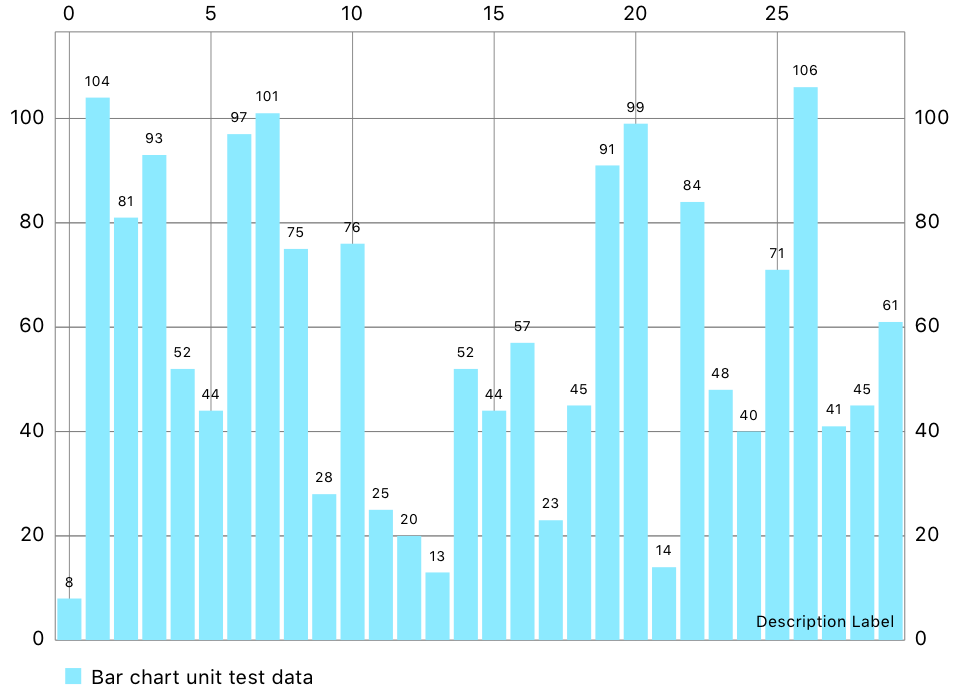
\includegraphics[width=10cm]{images/bodies/thirdparty/case/testDefaultValues.png}
    \caption{スクリーンショットを用いたテストと対応する画像}
    \label{figure:danielgindi/Charts:d300d6d:Tests/ReferenceImages_64/ChartsTests.BarChartTests/testDefaultValues_iOS_320.0_568.0@2x.png}
\end{figure}

ios-snapshot-test-caseを利用しているライブラリとしては次のようなものがある.括弧内は確認したコミット番号である.

\begin{itemize}
    \item \href{https://github.com/facebookarchive/AsyncDisplayKit}{facebookarchive/AsyncDisplayKit: Smooth asynchronous user interfaces for iOS apps.}(5df7456c56e3fd579783b8816aacb82cc6c1abd1)
    \item \href{https://github.com/dzenbot/DZNEmptyDataSet}{dzenbot/DZNEmptyDataSet: A drop-in UITableView/UICollectionView superclass category for showing empty datasets whenever the view has no content to display}(b5b9216d09f19455aa616d3bda32e1c38d3178bd)
    \item \href{https://github.com/danielgindi/Charts}{danielgindi/Charts: Beautiful charts for iOS/tvOS/OSX! The Apple side of the crossplatform MPAndroidChart.}(8245f32498739cde83dc729123d58538184b78f5)
\end{itemize}

ブログに紹介されている33個のライブラリのうちfastlaneを使用しているのは\href{https://github.com/onevcat/Kingfisher}{onevcat/Kingfisher: A lightweight, pure-Swift library for downloading and caching images from the web.}(037c3ec78bb77cb16a6f3076006f718fd66283c6)と\href{https://github.com/onevcat/Hedwig}{onevcat/Hedwig: Send email to any SMTP server like a boss, in Swift and cross-platform}(8e3b629982eb9f2576225400819482164b6e248d)の2個で,どちらもテストやGitHubへのリリースに使用しておりsnapshot機能は使用していない.


\section{ネットワーク通信を行うライブラリのテスト}\label{section:thirdparty_case_network}
ネットワークリクエストを行うライブラリはどのようにテストを行っているのだろうか.

\ref{chapter:thirdparty_framework}章ではネットワークリクエストスタブフレームワークの\href{https://github.com/AliSoftware/OHHTTPStubs}{AliSoftware/OHHTTPStubs: Stub your network requests easily! Test your apps with fake network data and custom response time, response code and headers!}を紹介した.\href{https://github.com/ishkawa/APIKit}{ishkawa/APIKit: Type-safe networking abstraction layer that associates request type with response type.}はOHHTTPStubs(のちに独自のスタブへ変更)を用いてテストを行っているライブラリである.変更の経緯については\ref{section:thirdparty_case_spm}節で述べる.

実際のサーバと通信を行ってテストを行うライブラリも存在する.\href{https://httpbin.org/}{httpbin(1): HTTP Client Testing Service}はHTTPリクエスト\&レスポンスサービスサイトで,エンドポイント毎にさまざまなレスポンスを返す.\href{https://github.com/Alamofire/Alamofire}{Alamofire/Alamofire: Elegant HTTP Networking in Swift}ではこのエンドポイントを利用してリクエストテストを行っている.プログラム\ref{lstlisting:Alamofire/Alamofire:c20e17e:Tests/RequestTests.swift:44-57}はパラメータとともにGETリクエストを行うテストである.リクエストに正しいパラメータが含まれているかどうか,レスポンスがあったかどうかをアサーションで確かめている.

\begin{lstlisting}[language=swift,caption=\href{https://github.com/Alamofire/Alamofire/blob/c20e17e38eadefbc6d77332290e5b7e84eb15932/Tests/RequestTests.swift}{Alamofireでのパラメータ付きGETリクエストテスト},label=lstlisting:Alamofire/Alamofire:c20e17e:Tests/RequestTests.swift:44-57,firstnumber=44]
    func testRequestClassMethodWithMethodAndURLAndParameters() {
        // Given
        let urlString = "https://httpbin.org/get"

        // When
        let request = Alamofire.request(urlString, parameters: ["foo": "bar"])

        // Then
        XCTAssertNotNil(request.request)
        XCTAssertEqual(request.request?.httpMethod, "GET")
        XCTAssertNotEqual(request.request?.url?.absoluteString, urlString)
        XCTAssertEqual(request.request?.url?.query, "foo=bar")
        XCTAssertNil(request.response)
    }
\end{lstlisting}

一方,メール送信ライブラリ\href{https://github.com/onevcat/Hedwig}{onevcat/Hedwig: Send email to any SMTP server like a boss, in Swift and cross-platform}ではライブラリ作者の所有するドメインからのメール送信を試みている.以前はnpmによるローカルサーバを使用していた.
% コミット: 485df427e36c0886e57a2070cdfc78b27ca2a131




\section{多言語プロジェクトにおけるテスト方針}\label{section:thirdparty_case_multilingualization}
iOSライブラリの中には多言語にまたがるプロジェクトのライブラリがある.

\href{https://promisesaplus.com/}{Promises/A+}は非同期処理表現promiseの公開基準で,\href{http://wiki.commonjs.org/wiki/Promises/A}{Promises/A - CommonJS Spec Wiki}の派生である.Promises/A+仕様はpromiseの{\sf then}メソッドを提供する一方で,create,fulfill,reject操作を扱うものではない\cite{promisesaplus.com}.\href{https://github.com/promises-aplus/promises-tests}{promises-aplus/promises-tests: Compliances tests for Promises/A+}リポジトリにあるテストに成功すれば,Promises/A+の定める{\sf then}メソッドが実装されているとしてREADMEにPromises/A+ロゴを掲載することができる\cite{github:promises-aplus/promises-tests}.図\ref{figure:promisesaplus.com:logo}はPromises/A+のロゴである.

\begin{figure}
    \centering
    
\includegraphics{images/bodies/thirdparty/case/promisesaplus_logo-small.png}
    \caption{Promises/A+のロゴ}
    \label{figure:promisesaplus.com:logo}
\end{figure}

\href{https://github.com/mxcl/PromiseKit}{mxcl/PromiseKit: Promises for Swift \& ObjC}はSwiftとObjective-Cにpromiseを提供するライブラリである.PromiseKitのテストにはA+,Bridging,CorePromiseの3種類があり,このうちのA+で\href{https://github.com/promises-aplus/promises-tests}{promises-aplus/promises-tests: Compliances tests for Promises/A+}のテストを行っている.ただしJavaScriptとSwiftの言語仕様の違いから一部の項目はスキップされている\cite{github:mxcl/PromiseKit:Tests/A+/README.md}.

\begin{lstlisting}[language=javascript,caption=\href{https://github.com/promises-aplus/promises-tests/blob/4bab3171e3aeb4b3612c84ef28c128eb430be0a6/lib/tests/2.1.2.js}{Promises/A+におけるテスト2.1.2.1},label=lstlisting:promises-aplus/promises-tests:4bab317:lib/tests/2.1.2.js:11-23,firstnumber=11]
describe("2.1.2.1: When fulfilled, a promise: must not transition to any other state.", function () {
    testFulfilled(dummy, function (promise, done) {
        var onFulfilledCalled = false;

        promise.then(function onFulfilled() {
            onFulfilledCalled = true;
        }, function onRejected() {
            assert.strictEqual(onFulfilledCalled, false);
            done();
        });

        setTimeout(done, 100);
    });
\end{lstlisting}

\begin{lstlisting}[language=swift,caption=\href{https://github.com/mxcl/PromiseKit/blob/b1dd2bf874002e7fa142cd0a1356528e204f5779/Tests/A+/2.1.2.swift}{PromiseKitにおけるテスト2.1.2.1},label=lstlisting:mxcl/PromiseKit:b1dd2bf:Tests/A+/2.1.2.swift:4-9,firstnumber=4]
class Test212: XCTestCase {
    func test() {
        describe("2.1.2.1: When fulfilled, a promise: must not transition to any other state.") {
            testFulfilled { promise, expectation, _ in
                promise.test(onFulfilled: expectation.fulfill, onRejected: { XCTFail() })
            }
\end{lstlisting}

プログラム\ref{lstlisting:promises-aplus/promises-tests:4bab317:lib/tests/2.1.2.js:11-23}はA+が定める2.1.2.1の,プログラム\ref{lstlisting:mxcl/PromiseKit:b1dd2bf:Tests/A+/2.1.2.swift:4-9}はPromiseKitで行われている2.1.2.1のテストコードの冒頭である.A+は\href{https://mochajs.org/}{Mocha - the fun, simple, flexible JavaScript test framework}の,PromiseKitは独自実装の{\sf describe}メソッドを用いてビヘイビア駆動のテストを行っている.


\section{テストコードの自動生成}\label{section:thirdparty_case_autogeneration}
ライブラリの中にはテストコードを自動生成しているものもある.ここでは\href{https://github.com/ReactiveX/RxSwift}{ReactiveX/RxSwift: Reactive Programming in Swift}を紹介する.

RxSwiftではPreprocessorターゲットにソースコード自動生成のプロジェクトを用意している.独自のプログラムにより*.ttファイルを*.swiftに変換する.パフォーマンス,一貫性のため,開発者を重荷から解放するため,そして楽しいからという理由による\cite{github:ReactiveX/RxSwift:Preprocessor/README.md}.*.ttファイル中では{\sf \textless\%= \%\textgreater}を用いてスクリプトを書くことができる.例えば,{\sf Observable}の{\sf zip}メソッドの場合,{\sf i = 2 \ldots 8}の範囲でプログラム\ref{lstlisting:ReactiveX/RxSwift:b32a0f0:RxSwift/Observables/Zip+arity.tt:22-29}からプログラム\ref{lstlisting:ReactiveX/RxSwift:b32a0f0:RxSwift/Observables/Zip+arity.swift:23-30}が生成される.テストメソッドについてもプログラム\ref{lstlisting:ReactiveX/RxSwift:b32a0f0:Tests/RxSwiftTests/Observable+ZipTests+arity.tt:14-20}のようなttファイルが用意されている.

\begin{lstlisting}[language=swift,caption=\href{https://github.com/ReactiveX/RxSwift/blob/b32a0f0d40656672783749d23e2984bf337adcec/RxSwift/Observables/Zip+arity.tt}{{\sf zip}メソッドのテンプレート},label=lstlisting:ReactiveX/RxSwift:b32a0f0:RxSwift/Observables/Zip+arity.tt:22-29,firstnumber=22]
    public static func zip<<%= (Array(1...i).map { "O\($0): ObservableType" }).joined(separator: ", ") %>>
        (<%= (Array(1...i).map { "_ source\($0): O\($0)" }).joined(separator: ", ") %>, resultSelector: @escaping (<%= (Array(1...i).map { "O\($0).E" }).joined(separator: ", ") %>) throws -> E)
        -> Observable<E> {
        return Zip<%= i %>(
            <%= (Array(1...i).map { "source\($0): source\($0).asObservable()" }).joined(separator: ", ") %>,
            resultSelector: resultSelector
        )
    }
\end{lstlisting}

\begin{lstlisting}[language=swift,caption=\href{https://github.com/ReactiveX/RxSwift/blob/b32a0f0d40656672783749d23e2984bf337adcec/RxSwift/Observables/Zip+arity.swift}{自動生成された{\sf zip}メソッド},label=lstlisting:ReactiveX/RxSwift:b32a0f0:RxSwift/Observables/Zip+arity.swift:23-30,firstnumber=23]
    public static func zip<O1: ObservableType, O2: ObservableType>
        (_ source1: O1, _ source2: O2, resultSelector: @escaping (O1.E, O2.E) throws -> E)
        -> Observable<E> {
        return Zip2(
            source1: source1.asObservable(), source2: source2.asObservable(),
            resultSelector: resultSelector
        )
    }
\end{lstlisting}

\begin{lstlisting}[language=swift,caption=\href{https://github.com/ReactiveX/RxSwift/blob/b32a0f0d40656672783749d23e2984bf337adcec/Tests/RxSwiftTests/Observable+ZipTests+arity.tt}{{\sf zip}メソッドのテストテンプレート},label=lstlisting:ReactiveX/RxSwift:b32a0f0:Tests/RxSwiftTests/Observable+ZipTests+arity.tt:14-20,firstnumber=14]
extension ObservableZipTest {
<% for i in 2 ... 8 { %>

    // <%= i %>

    func testZip_ImmediateSchedule<%= i %>() {
        let factories: [(<%= (Array(0..<i).map { _ in "Observable<Int>" }).joined(separator: ", ") %>) -> Observable<Int>] =
\end{lstlisting}

ソースコードを自動生成しているライブラリには他にも\href{https://github.com/thoughtbot/Curry}{thoughtbot/Curry: Swift implementations for function currying}があるが,Curryはテストを行っていない.なお,RxSwiftもCurryも関数型プログラミングの考え方が背景にあるライブラリである.



\section{Swift Package ManagerとLinux対応}\label{section:thirdparty_case_spm}
Swift Package Manager,ひいてはLinuxへの各ライブラリの対応を紹介する.

\ref{section:thirdparty_case_network}節でAPIKitがOHHTTPStubsの使用を取りやめたことを紹介した.これは,Swift Package Managerをサポートするにあたり,OHHTTPStubsがCocoaPodsとCarthageのみの対応でSwift Package Managerでインストールできないためである.そこで,APIKitではswift testコマンドを実行できるよう機能縮小した独自の{\sf HTTPStub}へ変更した\cite{github:ishkawa/APIKit:130}\cite{github:ishkawa/APIKit:209}.

Swift Package Managerに対応しながらもテストを除外しているライブラリもある.このようなライブラリでは,.xcodeprojにのみテストファイルを登録し,Package.swiftからは除外している.プログラム\ref{lstlisting:Alamofire/Alamofire:b899544:Package.swift:27}はAlamofireのPackage.swiftの,プログラム\ref{lstlisting:onevcat/Kingfisher:3b76bc6:Package.swift:29-32}はKingfisherのPackage.swiftである.Kingfisherではテストの他にUIKitに関係するSwiftファイルも除外している.

\begin{lstlisting}[language=swift,caption=\href{https://github.com/Alamofire/Alamofire/blob/b8995447518fd57af14c88a47f27434a16f60403/Package.swift}{Alamofireのパッケージ設定},label=lstlisting:Alamofire/Alamofire:b899544:Package.swift:27,firstnumber=27]
let package = Package(name: "Alamofire", dependencies : [], exclude: ["Tests"])
\end{lstlisting}

\begin{lstlisting}[language=swift,caption=\href{https://github.com/onevcat/Kingfisher/blob/3b76bc6ca9f56d5fd5635439eda9318eff7945e3/Package.swift}{Kingfisherのパッケージ設定},label=lstlisting:onevcat/Kingfisher:3b76bc6:Package.swift:29-32,firstnumber=29]
let package = Package(
  name: "Kingfisher",
  exclude: ["Tests","Sources/AnimatedImageView.swift","Sources/UIButton+Kingfisher.swift"]
)
\end{lstlisting}





%------------------------------%

\newgeometry{hmarginratio=1:1}
\begin{appendices}
\restoregeometry
\chapter{ソフトウェアテスト用語集}
% TODO: fix
\thispagestyle{fancy}
本付録ではISO/IEC/IEEE 29119\cite{ieee29119-1}\cite{ieee29119-2}\cite{ieee29119-3}\cite{ieee29119-4}\cite{ieee29119-5}で定められるソフトウェアテストの用語を紹介する.用語の日本語訳はJSTQB®技術委員会の翻訳\cite{jstqb_words}に従う.

\begin{description}
    \item[accessibility testing(アクセシビリティテスト)\index{accessibility testing}]usability testingの一種.障害者を含む多くのユーザがtest itemを使えるかどうかを測る.
    \item[actual results(実行結果)\index{actual results}]test executionの結果として観測される,test itemの振る舞いや状態の集合,関連するデータやtest environmentの状態の集合のこと.例えば,ハードウェアへの出力,データの変更,レポート,メッセージの送信がある.
    \item[backup and recovery testing\index{backup and recovery testing}]reliability testingの一種.時間,コスト,完全性,故障事例の確実性といった特定の状況下でシステムの状態をバックアップから復元できるかどうかを測定するテスト.
    \item[Backus-Naur Form\index{Backus-Naur Form}]テキスト形式において,言語の構文の定義に用いられる形式的なメタ言語
    \item[base choice\index{base choice}]→base value
    \item[black-box testing(ブラックボックステスト)\index{black-box testing}]→specification-based testing
    \item[c-use\index{c-use}]→computation data use
    \item[capacity testing\index{capacity testing}]performance efficiency testingの一種.ユーザ,トランザクション,データストレージのような負荷の上昇に対し,要求されるパフォーマンスを維持する能力を損なうレベルを測定する.
    \item[compatibility testing(互換性テスト)\index{compatibility testing}]共通の環境(co-existence)や,必要に応じて他のシステムやコンポーネントと情報交換をする状態(interoperability)において,他の独立したプロダクトと共にtest itemが満足に作用するかどうかを測定するテスト.
    \item[completion criteria(終了基準)\index{completion criteria}]テストの処理が完了したと見なされる条件のこと.
    \item[computation data use\index{computation data use}]任意の種類のステートメントにおける,変数の値の使用
    \item[condition(条件)\index{condition}]論理演算子を含まない論理式のこと.{\sf A < B}はconditionだが{\sf A and B}はconditionではない.
    \item[control flow(制御フロー)\index{control flow}]test itemの実行中に処理が実行されるシーケンス.
    \item[control flow sub-path\index{control flow sub-path}]test item中のexectabule statementのシーケンス.
    \item[coverage item(カバレッジアイテム)\index{coverage item}]→test coverage item
    \item[data definition(データ定義)\index{data definition}]値を変数に割り当てるステートメント.別名: variable definition\index{variable definition}.
    \item[data definition c-use pair\index{data definition c-use pair}]data definition及び,後続のcomputation data useでdata useがdata definitionで定義された値を使うもののこと.
    \item[data definition p-use pair\index{data definition p-use pair}]data definition及び,後続のpredicate data useでdata useがdata definitionで定義された値を使うもののこと.
    \item[data definition-use pair\index{data definition-use pair}]data definition及び,後続のdata useでdata useがdata definitionで定義された値を使うもののこと.
    \item[data use\index{data use}]変数の値にアクセスするexecutable statementのこと.
    \item[decision(判定)\index{decision}]処理の集合の出力として考えうる2つ以上の出力のうちどちらかを選ぶ状態のこと.if-then-elseのような単純な選択や,while-loopのようなループをいつ脱出するかの決定,case-1-2-3-..-Nのようなcase(switch)文のこと.
    \item[decision outcome(判定結果)]decisionの結果のこと.これに従ってcontrol flowがどちらに進むかが決まる.
    \item[decision rule\index{decision rule}]decision table testingやcause-effect graphingにおいて,特定の出力を出力するconditionの組み合わせ(= causes)と処理(= effects)のこと.
    \item[definition-use pair(定義使用ペア)\index{definition-use pair}]data definition及び,後続のpredicate/computational data useでdata useがdata definitionで定義された値を使うもののこと.
    \item[domain layer\index{domain layer}]test itemの抽象化の最高レベルのこと.Note 1 to entry: Keywords on this level are chosen in a way that is familiar to domain experts.
    \item[dynamic testing(動的テスト)\index{dynamic testing}]test itemの実行を必要とするテストのこと.
    \item[endurance testing(耐久テスト)\index{endurance testing}]performance efficiency testingの一種で,test itemが特定の時間の間必要な読み込みを継続的に行えるかどうか確かめるテスト.
    \item[entry point(開始点)\index{entry point}]test itemの実行を開始できるポイントのこと.entry pointはtest item中の1つ以上のpathの開始点として外部プロセスに選択される,test item内のexectable statementである.大抵はtest item中の最初のexecutable statementである.
    \item[equivalence partition(同値分割)\index{equivalence partition}]同じ区分の全ての値がtest itemによって同様に扱われることが合理的に期待できるような,test itemの範囲内や境界面の変数の変域の部分集合や変数の集合
    \item[equivalence partition coverage(同値分割カバレッジ)\index{equivalence partition coverage}]test setによってカバーされるtest itemの,同一と見なされた同値分割の割合.多くの場合,同値分割の同一確認は(無効な分割の部分分割においては特に)主観的である.よって,test item内の同値分割数の決定的な勘定は不可能である.
    \item[equivalence partitioning(同値分割法)\index{equivalence partitioning}]test design techniqueの1つで,各同値クラス内の1つ以上の代表値を用いることで,equivalence partitionsを実行するテストを用意すること.
    \item[error guessing(エラー推測)\index{error guessing}]テスターの過去の失敗の経験や,失敗の様式の一般的な知識といったものをベースに行うtest design technique.関連する知識は個人的な経験から得られたり,欠陥データベースやバグの分類に要約されたりする.
    \item[executable statement(実行ステートメント)\index{executable statement}]コンパイルされた時にオブジェクトコードに翻訳され,test itemが実行されプログラムデータ上でアクションを起こすだろう時に手続き的に実行されるステートメントのこと.
        statement which, when compiled, is translated into object code, which will be executed procedurally when the test item is running and may perform an action on program data
    \item[exit point(終了点)\index{exit point}]test item中の最後のexecutable statementのこと.entry pointはtest item中のpathの終点で、test itemを停止させるか外部プロセスに制御を戻すようなexecutable statementである.一般的にはtest item中の最後のexecutable statementである.
    \item[expected results(期待結果)\index{expected results}]仕様や別のソースをもとにした特定の状態の下のtest itemの,観測可能で予想される振る舞い
    \item[exploratory testing(探索的テスト)\index{exploratory testing}]experience-based testingの一種.テスターの関連知識やテストアイテムの事前の探索(前回のテストの結果を含む),一般的なソフトウェアの振る舞いと失敗の種類に対するヒューリスティックな"大まかなやり方"をベースにしてテスターが自発的にテストをデザインし実行するもの.exploratory testingは,温和である可能性がかなり高いと同時に,テスト中ソフトウェアの他のプロパティを邪魔するためにソフトウェアが失敗するリスクを生み出す隠れたプロパティ(隠れた振る舞いを含む)を探す.
    \item[feature set\index{feature set}]リスクや要求,機能,モデルから集めることのできるテスト対象のtest itemのtest conditionを含むアイテムの集合.これは,そのアイテムの全ての機能の集合(full feature set)の場合や,特定の目的のために識別された部分集合(functional feature set)の場合がある.
    \item[high-level keyword\index{high-level keyword}]keyword that covers complex activities that may be composed from other keywords and is used by domain experts to assemble keyword test cases
    \item[Incident Report(インシデントレポート)\index{Incident Report}]インシデントの発生,性質,ステータスのドキュメント
    \item[installability testing(設置性テスト)\index{installability testing}]portability testingの一種.test itemやその集合が全ての指定の環境でインストールできることを確認するテスト
    \item[keyword\index{keyword}]one or more words used as a reference to a specific set of actions intended to be performed during the execution of one or more test cases.Note 1 to entry: The actions include interactions with the User Interface during the test, verification, and specific actions to set up a test scenario.Note 2 to entry: Keywords are named using at least one verb.Note 3 to entry: Composite keywords can be constructed based on other keywords.
    \item[keyword dictionary\index{keyword dictionary}]repository containing a set of keywords reflecting the language and level of abstraction used to write test cases
    \item[Keyword-Driven Testing(キーワード駆動テスト)\index{Keyword-Driven Testing}]testing using test cases composed from keywords
    \item[Keyword-Driven Testing framework\index{Keyword-Driven Testing framework}]test framework covering the functional capabilities of a keyword-driven editor, decomposer, data sequencer, manual test assistant, tool bridge, data and script repositories, a keyword library and the test execution environment
    \item[keyword execution code\index{keyword execution code}]implementation of a keyword that is intended to be executed by a test execution engine
    \item[keyword library\index{keyword library}]→keyword dictionary
    \item[keyword test case\index{keyword test case}]sequence of keywords and the required values for their associated parameters (as applicable) that are composed to describe the actions of a test case
    \item[load testing(ロードテスト)\index{load testing}]performance efficiency testingの一種で,変動する負荷の予想される条件下でのtest itemの振る舞いを評価する.通常は低,標準,ピーク使用といった予想される条件の間で行う.
    \item[low-level keyword\index{low-level keyword}]keyword that covers only one or very few simple actions and is not composed from other keywords
    \item[maintainability testing(保守性テスト)\index{maintainability testing}]改修される可能性のあるtest itemに対して有効性や効率の度合いを評価するために実施されるようなtest type
    \item[manual testing\index{manual testing}]人間がtest itemに情報を入力したり結果を検証したりして行うテストのこと.automated testing\index{automated testing}ではツールやロボットや他のtest execution engineを用いてテストする.manual testingではこういったアイテムを使用しない.
    \item[Organizational Test Policy\index{Organizational Test Policy}]組織におけるテストの目的や目標,全体的なスコープを記述し,テストを行う理由と達成すべき事柄を示した実行レベルのドキュメントのこと.Note 1 to entry: It is generally preferable to keep the Organizational Test Policy as short as possible in a given context.
    \item[Organizational Test Process\index{Organizational Test Process}]organizational test specificationを開発し管理するためのtest process
    \item[organizational test specification\index{organizational test specification}]組織におけるテストに関する情報,つまりプロジェクト固有ではない情報を示す文書.EXAMPLE organizational test specificationの一般的な例は,Organizational Test PolicyとOrganizational Test Strategyである.
    \item[Organizational Test Strategy\index{Organizational Test Strategy}]組織内で実行される全プロジェクトで扱われるテストの一般的な要件を示す文書で,テストの実行方法の詳細が記載されている.Note 1 to entry: The Organizational Test Strategy is aligned with the Organizational Test Policy.Note 2 to entry: An organisation could have more than one Organizational Test Strategy to cover markedly different project contexts.
    \item[p-use\index{p-use}]→predicate data use
    \item[P-V pair\index{P-V pair}]→test itemのパラメータとそれに割り当てた値の組み合わせのこと.combinational test design technique\index{combinational test design technique}でtest conditionとcoverage itemとして用いる.
    \item[pass/fail criteria(合格/失敗基準)\index{pass/fail criteria}]テスト後にtest itemやその機能が合格か失敗かを決定するのに使われるdecision ruleのこと.
    \item[path(パス)\index{path}]→test itemのexecutable statementsのシーケンスのこと.
    \item[performance testing(性能テスト)\index{performance testing}]与えられた時間や資源の制約の中で,指定された機能をtest itemが達成できる度合いを評価するために行うテストの種類
    \item[portability testing(移植性テスト)\index{portability testing}]1つのハードウェアまたはソフトウェアの環境から別のハードウェアまたはソフトウェア環境にtest itemを移動させる際の容易さを評価するために行われるtestの種類で,様々な種類の環境で実行するために必要な変更のレベルを含む.
    \item[predicate(プレディケート)\index{predicate}]{\sf TRUE}または{\sf FALSE}と評価される論理式のことで,通常はコード中の実行パスを指し示す.
    \item[predicate data use\index{predicate data use}]判定ステートメントの述語部分のdecision outcomeに関連するdata use
    \item[procedure testing(手続きテスト)\index{procedure testing}]test itemやその出力に対する相互作用の手続き命令がユーザの要求を満たし使用目的をサポートしているかを評価するために行われる,functional suitability testingの一種.
    \item[product risk(プロダクトリスク)\index{product risk}]機能,品質,構造の特定の側面において製品に欠陥のある可能性があるようなリスク
    \item[project risk(プロジェクトリスク)\index{project risk}]プロジェクトのマネジメントに関係するリスク.EXAMPLE 人員の不足,厳しい期限,要件の変更.
    \item[regression testing(回帰テスト)\index{regression testing}]回帰失敗が起きるかどうかを識別するための,test itemや運用環境の変更に続くテスト.Note 1 to entry: The sufficiency of a set of regression test cases depends on the item under test and on the modifications to that item or its operational environment.
    \item[reliability testing(回復性テスト)\index{reliability testing}]規定の条件のもとで特定期間使用された時に,故障が発生する頻度やtest itemが要求される機能を果たす能力を評価するために行われるtestの一種.
    \item[retesting\index{retesting}]以前に"fail"の結果を返したtest caseを再実行し是正措置の効果を評価すること.Note 1 to entry: Also known as confirmation testing\index{confirmation testing}.
    \item[risk-based testing(リスクベースドテスト)\index{risk-based testing}]testing in which the management, selection, prioritisation, and use of testing activities and resources are consciously based on corresponding types and levels of analyzed risk
    \item[scenario testing(シナリオテスト)\index{scenario testing}]class of test design technique in which tests are designed to execute individual scenarios.Note 1 to entry: A scenario can be a user story, use-case, operational concept, or sequence of events the software may encounter etc.
    \item[scripted testing(スクリプトテスト)\index{scripted testing}]dynamic testingの一種.テスターの操作がtest caseの中の指示書に事前に記述されている.この用語は通常スクリプトで自動で実行されるテストよりも手動で実行されるテストに適用される.
    \item[security testing(セキュリティテスト)\index{security testing}]type of testing conducted to evaluate the degree to which a test item, and associated data and information, are protected so that unauthorized persons or systems cannot use, read, or modify them, and authorized persons or systems are not denied access to them
    \item[specification-based testing(仕様ベースドテスト)\index{specification-based testing}]testing in which the principal test basis is the external inputs and outputs of the test item, commonly based on a specification, rather than its implementation in source code or executable software.Note 1 to entry: Synonyms for specification-based testing include black-box testing and closed box testing.
    \item[statement coverage(ステートメントカバレッジ)\index{statement coverage}]test setによってカバーされた,test itemの全てのexecutable statementの集合の割合のこと.
    \item[statement testing(ステートメントテスト)\index{statement testing}]test design technique in which test cases are constructed to force execution of individual statements in a test item
    \item[static testing(静的テスト)\index{static testing}]コードを実行せずに,品質や他の基準についてtest itemを検査するtestingのこと.レビューや静的解析など.
    \item[stress testing(ストレステスト)\index{stress testing}]type of performance efficiency testing conducted to evaluate a test item's behaviour under conditions of loading above anticipated or specified capacity requirements, or of resource availability below minimum specified requirements
    \item[structural testing(構造テスト)\index{structural testing}]→structure-based testing
    \item[structure-based testing(構造ベースドテスト)\index{structure-based testing}]dynamic testing in which the tests are derived from an examination of the structure of the test item.Note 1 to entry: Structure-based testing is not restricted to use at component level and can be used at all levels, e.g. menu item coverage as part of a system test.Note 2 to entry: Techniques include branch testing, decision testing, and statement testing.Note 3 to entry: Synonyms for structure-based testing are structural testing, glass-box testing, and white box testing.
    \item[sub-path(サブパス)\index{sub-path}]より大きなpathの一部のpathのこと.
    \item[suspension criteria(中止基準)\index{suspension criteria}]criteria used to (temporarily) stop all or a portion of the testing activities
    \item[test basis(テストベース)\index{test basis}]body of knowledge used as the basis for the design of tests and test cases.Note 1 to entry: The test basis may take the form of documentation, such as a requirements specification, design specification, or module specification, but may also be an undocumented understanding of the required behaviour.
    \item[test case(テストケース)]test caseの前提条件,入力(適用できる場合はアクションを含む),expected resultの集合で,適切な実装やエラーの識別,品質検査,その他の重要な情報を含むtestの目的の達成のためにtest itemを実行するべく開発される.Note 1 to entry: test caseは意図するtest sub-processに対するtest入力の最も低いレベル(つまりtest caseはtest caseで構成されていない)である.Note 2 to entry: test caseの前提条件にはtest environment,既存のデータ(データベースなど),test対象のソフトウェア,ハードウェアなどが含まれる.Note 3 to entry: 入力はtest executionを実行するために用いられるデータ情報である.Note 4 to entry: expected resultには成功基準や確認すべき失敗などが含まれる.
    \item[Test Case Specification(テストケース仕様)\index{Test Case Specification}]documentation of a set of one or more test cases
    \item[Test Completion Process\index{Test Completion Process}]Test Management Process for ensuring that useful test assets are made available for later use, test environments are left in a satisfactory condition, and the results of testing are recorded and communicated to relevant stakeholders
    \item[Test Completion Report\index{Test Completion Report}]report that provides a summary of the testing that was performed.Note 1 to entry: Also known as a Test Summary Report.
    \item[test condition(テスト条件)\index{test condition}]testable aspect of a component or system, such as a function, transaction, feature, quality attribute, or structural element identified as a basis for testing.Note 1 to entry: Test conditions can be used to derive coverage items, or can themselves constitute coverage items.
    \item[test coverage(テストカバレッジ)\index{test coverage}]test caseによって実行された特定のtest coverage itemの割合で,パーセントで表される.
    \item[test coverage item\index{test coverage item}]test executionの徹底度合いを測定できるようにするためにtest design techniqueに使われた,1つ以上のtest conditionに由来する属性または属性の集合のこと.
    \item[test data(テストデータ)\index{test data}]1つ以上のtest caseを実行するために入力条件を満たすために作られるか選ばれるデータで,Test Planやtest case,test procedureで定義される.test dataはテスト下のプロダクトとともに(配列やファイル,データベースの形で)保存されるか,他のシステムやそのコンポーネント,ハードウェアデバイス,人間の操作によって与えられる.
    \item[Test Data Readiness Report\index{Test Data Readiness Report}]document describing the status of each test data requirement
    \item[Test Design and Implementation Process\index{Test Design and Implementation Process}]test process for deriving and specifying test cases and test procedures
    \item[Test Design Specification(テスト設計仕様)\index{Test Design Specification}]document specifying the features to be tested and their corresponding test conditions
    \item[test design technique(テスト設計技法)\index{test design technique}]activities, concepts, processes, and patterns used to construct a test model that is used to identify test conditions for a test item, derive corresponding test coverage items, and subsequently derive or select test cases
    \item[test environment(テスト環境)\index{test environment}]facilities, hardware, software, firmware, procedures, and documentation intended for or used to perform testing of software.Note 1 to entry: A test environment could contain multiple environments to accommodate specific test sub-processes (e.g. a unit test environment, a performance test environment etc.).
    \item[test environment readiness report\index{test environment readiness report}]document that describes the fulfilment of each test environment requirement
    \item[Test Environment Requirements\index{Test Environment Requirements}]description of the necessary properties of the test environment.Note 1 to entry: All or parts of the test environment requirements could reference where the information can be found, e.g. in the appropriate Organizational Test Strategy, Test Plan, and/or Test Specification.
    \item[Test Environment Set-up Process\index{Test Environment Set-up Process}]dynamic test process for establishing and maintaining a required test environment
    \item[test execution(テスト実行)\index{test execution}]test itemに対してテストを実行してactual resultを得ること.
    \item[test execution engine\index{test execution engine}]test caseを実行するためにtest itemを操作する,ソフトウェアやハードウェアに実装されているツール.典型的なtest execution engineはunit test tool framework,stimulation-command system,capture and playback toolや操作のためのソフトウェアが付属したhardware robotを含む.
    \item[Test Execution Log\index{Test Execution Log}]document that records details of the execution of one or more test procedures
    \item[Test Execution Process\index{Test Execution Process}]dynamic test process for executing test procedures created in the Test Design and Implementation Process in the prepared test environment, and recording the results
    \item[test framework\index{test framework}]テストを容易にする環境のこと.
    \item[Test Incident Reporting Process\index{Test Incident Reporting Process}]dynamic test process for reporting to the relevant stakeholders issues requiring further action that were identified during the test execution process
    \item[test interface\index{test interface}]interface to the test item used to stimulate the test item, to get responses (e.g. actual results), or both.Note 1 to entry: The GUI, API or SOA interfaces are typical test interfaces.Note 2 to entry: Stimulating the test item can involve passing data into it via computer interfaces or attached hardware. Note 3 to entry: Getting responses includes getting information from the test item under test or associated hardware.
    \item[test interface layer\index{test interface layer}]lowest level of abstraction for keywords, which interacts with the test item directly and encapsulates the atomic (lowest level) interactions at the test interface
    \item[test item(テストアイテム)\index{test item}]テスト対象の作業成果物.システムやソフトウェアアイテム,要求仕様書,設計仕様書,ユーザガイドなど.
    \item[test level(テストレベル)\index{test level}] test sub-processの具体的なインスタンス化.次にあげたものはtest sub-processとしてインスタンス化される一般的なtest levelである: component test level/sub-process,integration test level/sub-process,system test level/sub-process,acceptance test level/sub-process.test levelはtest phaseの代名詞である.
    \item[test management(テストマネジメント)\index{test management}]planning, scheduling, estimating, monitoring, reporting, control and completion of test activities
    \item[Test Management Process\index{Test Management Process}]test process containing the sub-processes that are required for the management of a test project.Note 1 to entry: See Test Planning Process, Test Monitoring and Control Process, Test Completion Process.
    \item[test model\index{test model}]representation of a test item that is used during the test case design process
    \item[Test Monitoring and Control Process\index{Test Monitoring and Control Process}]Test Management Process for ensuring that testing is performed in line with a Test Plan and with organizational test specifications
    \item[test object(テスト対象)\index{test object}]→test item
    \item[test phase(テストフェーズ)\index{test phase}]specific instantiation of test sub-process.Note 1 to entry: Test phases are synonymous with test levels, therefore examples of test phases are the same as for test levels (e.g. system test phase/sub-process).
    \item[Test Plan(テスト計画)\index{Test Plan}]detailed description of test objectives to be achieved and the means and schedule for achieving them, organised to coordinate testing activities for some test item or set of test items.Note 1 to entry: A project can have more than one Test Plan, for example there could be a Project Test Plan (also known as a master test plan) that encompasses all testing activities on the project; further detail of particular test activities could be defined in one or more test sub-process plans (i.e. a system test plan or a performance test plan).Note 2 to entry: Typically a Test Plan is a written document, though other plan formats could be possible as defined locally within an organization or project.Note 3 to entry: Test Plans could also be written for non-project activities, for example a maintenance test plan.
    \item[Test Planning Process\index{Test Planning Process}]Test Management Process used to complete test planning and develop Test Plans
    \item[Test Policy(テストポリシー)\index{Test Policy}]an executive-level document that describes the purpose, goals, principles and scope of testing within an organization.Note 1 to entry: The Test Policy defines what testing is performed and what it is expected to achieve but does not detail how testing is to be performed.Note 2 to entry: The Test Policy can provide a framework for establishing, reviewing and continually improving the organisations testing.
    \item[test practice\index{test practice}]conceptual framework that can be applied to the Organizational Test Process, the Test Management Process, and/or the Dynamic Test Process to facilitate testing.Note 1 to entry: Test Practices are sometimes referred to as test approaches.
    \item[test procedure(テスト手順)\index{test procedure}]実行順序におけるtest caseのシーケンスと,最初の初期条件のセットアップで必要になる関連する処理,実行後の処理をまとめるもののこと.test procedureは,連続して実行するために選んだ1つ以上のtest caseの集合の実行方法の詳細な指示を含む.sequence of test cases in execution order, and any associated actions that may be required to set up the initial preconditions and any wrap up activities post execution.Note 1 to entry: Test procedures include detailed instructions for how to run a set of one or more test cases selected to be run consecutively, including set up of common preconditions, and providing input and evaluating the actual result for each included test case.
    \item[Test Procedure Specification(テスト手順仕様)\index{Test Procedure Specification}]document specifying one or more test procedures, which are collections of test cases to be executed for a particular objective.Note 1 to entry: The test cases in a test set are listed in their required order in the test procedure..Note 2 to entry: Also known as a manual test script. A test procedure specification for an automated test run is usually called a test script.
    \item[test process(テストプロセス)\index{test process}]しばしば多くのアクティビティからなり,1つ以上のtest sub-processに分割される,ソフトウェアプロダクトの品質に関する情報を提供する.provides information on the quality of a software product, often comprised of a number of activities, grouped into one or more test sub-processes.特定のプロジェクトのtest processはシステムtest sub-processやtest planning sub-process(より大きなtest management processの一部),static testing sub-processといった複数のサブプロセスから構成されることもありうる.
    \item[test requirement(テスト要件)\index{test requirement}]→test condition
    \item[test result(テスト結果)\index{test result}]特定のtest caseが成功したか失敗したか,つまりtest itemの出力として観察されたactual resultがexpected resultに対応するかどうかや逸脱が観察されるかどうかを示すもの.
    \item[test script(テストスクリプト)\index{test script}]manual/automated testingのためのtest procedure specification.
    \item[test set(テストセット)\index{test set}]1つまたはそれ以上のtest caseとその実行に対する一般的な制約の集合のこと.特定のtest environment.特殊なドメイン知識,特定の目的など.
    \item[test specification(テスト仕様書)\index{test specification}]complete documentation of the test design, test cases and test procedures for a specific test item.Note 1 to entry: A test specification could be detailed in one document, in a set of documents, or in other ways, for example in a mixture of documents and database entries.
    \item[test specification technique(テスト仕様化技法)\index{test specification technique}]→test design technique
    \item[test status report\index{test status report}]report that provides information about the status of the testing that is being performed in a specified reporting period
    \item[test strategy(テスト戦略)\index{test strategy}]特定のtestプロジェクトやtest sub-processに対するtesting方法を示したTest Planの一部のこと.Note 1 to entry: test strategyはOrganizational Test Strategyとは別のエンティティである.Note 2 to entry: test strategyは通常次のいくつかまたは全てを記述する: 用いるtest practice,実装されたtest sub-process,採用するretestingとregression testing,用いるtest design techniqueと対応するtest完了基準,test data,test environmentとtestingツールの要件,test成果物に対する期待.
    \item[test sub-process\index{test sub-process}]一般的にtest projectの全test process内にある,特定のtest level(システムテスト,acceptance testingなど)やtest type(usability testing,performance testingなど)を行うために使うtest managementとdynamic/static test processのこと.test sub-processは1つまたはそれ以上のtest typeを含む.ライフサイクルモデルに頼ると,test sub-processは一般的にtest phase,test level,test stage,test taskと呼ばれる.
    \item[test technique(テスト技法)\index{test technique}]→test design technique
    \item[test traceability matrix\index{test traceability matrix}]document, spreadsheet, or other automated tool used to identify related items in documentation and software, such as requirements with associated tests.別名verification cross reference matrix\index{verification cross reference matrix},requirements test matrix\index{requirements test matrix},requirements verification table\index{requirements verification table}など.異なるtest traceability matrixは異なる情報,フォーマット,詳細のレベルを含む.
    \item[test type(テストタイプ)\index{test type}]特定の品質特性に着目したtesting activitiesの集合.test typeは1つのtest sub-processで行われるか,たくさんのtest sub-process(performance testingがcomponent test sub-processやsystem test sub-processとともに行われるなど)を横断して行われる.たとえば,security testing,functional testing,useability testing,performance testingなど.
    \item[testing(テスト)\index{testing}]1つ以上のtest itemの特性の発見や評価を容易にするために行う一連のアクティビティのこと.Note 1 to entry: testingアクティビティには,それがtestingに対するものである限り,計画や準備,実行,行動,マネージメントといったアクティビティが含まれる.
    \item[testware(テストウェア)\index{testware}]artefacts produced during the test process required to plan, design, and execute tests.Note 1 to entry: Testware can include such things as documentation, scripts, inputs, expected results, files, databases, environment, and any additional software or utilities used in the course of testing.
    \item[unscripted testing\index{unscripted testing}]dynamic testingの一種で,事前にtest case中にテスターの行動を記さないもののこと.
    \item[variable definition\index{variable definition}]→data definition
    \item[volume testing(ボリュームテスト)\index{volume testing}]volume testing type of performance efficiency testing conducted to evaluate the capability of the test item to process specified volumes of data (usually at or near maximum specified capacity) in terms of throughput capacity, storage capacity, or both
    \item[white box testing(ホワイトボックステスト)\index{white box testing}]→structure-based testing
\end{description}



\end{appendices}

\printbibheading[heading=bibintoc,title={参考文献}]
\thispagestyle{plain}
\printbibliography[heading=subbibintoc,type=article,title={Articles}]
\printbibliography[heading=subbibintoc,type=book,title={Books}]
\printbibliography[heading=subbibintoc,type=online,title={Onlines}]
\printbibliography[heading=subbibintoc,type=github,title={GitHubs}]

\printindex

\end{document}

